\chapter{Technical background}
\label{ch:TechBackground}

This chapter presents the technical background necessary to understand the design and implementation of the \acs{FPGA} verification platform. It begins with an examination of the Zynq UltraScale+ \acs{MPSoC} architecture, which serves as the primary technology for the servo drive control board. Subsequent sections address key implementation topics, including clocking strategies and clock-domain crossing management. The chapter concludes with an overview of various \acs{FPGA} verification methods, emphasizing in-system testing and the \acs{AMBA} \acs{AXI} protocols that are essential for the platform's communication infrastructure.

\section{Zynq UltraScale+ \acs{MPSoC} \acs{FPGA}}
\label{sec:TechBackground:Zynq_UltraScale+_MPSoc} 
Organizations developing advanced intelligent systems that leverage both hardware and software programmability can accelerate product development, increase value, and continuously enhance their products through flexibility, reuse, and rapid upgrades. In response to these evolving requirements, Xilinx introduced the UltraScale \acs{MPSoC} architecture. This platform builds on the earlier 28-nanometer Zynq-7000 All Programmable \acs{SoC} and UltraScale \acs{FPGA} families to address the higher performance and functionality demanded by next-generation applications \cite{XilinxUltraScaleMPSoCArchitecture}.

Essential features of Zynq UltraScale+ \acs{MPSoC} include \cite{XilinxUltraScaleMPSoCArchitecture}:
\begin{enumerate}
	\item \textbf{ Optimized Processing Engines for Specific Tasks:}
	This architecture employs both hardware and software processing engines to address bottlenecks in digital signal processing, graphics, networking, real-time control, and general computing. The heterogeneous processor mix enhances efficiency in terms of performance, power consumption, and cost.
	\item \textbf{ Scalability to 64-Bit Processing:}
	Processing capabilities scale from 32-bit to 64-bit and fully support virtualization. The system interconnect, peripherals, and memory architecture provide a large address space, enabling future scalability.
	\item \textbf{Advanced Interconnect and Memory Architecture:}
	A high-speed interconnect and advanced memory system enable all processing engines to share data efficiently, minimizing latency and maintaining optimal system performance.
	\item \textbf{ \acs{FPGA} Scalability and ASIC-Class Performance:}
	Programmable logic with ASIC-like features enables hardware acceleration for demanding tasks. The Vivado design tools facilitate real-time performance and rapid hardware customization.
	\item \textbf{ Multi-Level Security, Safety, and Reliability:}
	The architecture incorporates robust anti-tamper protections, trust features, and reliable operation, making it suitable for Internet of Things and mission-critical applications in challenging environments.
	\item \textbf{ Advanced Power Management:}
	Granular power control across processors enables the system to adjust power consumption dynamically, reducing both idle and active power according to workload demands.
	\item \textbf{ 16nm FinFET Performance per Watt Advantage:}
	Utilizing TSMC 16nm FinFET technology, UltraScale \acs{MPSoC}s deliver up to 60\% improved performance per watt compared to 28nm devices, while mitigating the risks associated with custom ASIC development.
	\item \textbf{  High-Level Design Abstractions:}
	Support for C/C++, SystemC, OpenCL, MATLAB, and other tools makes it easy to speed up software-to-hardware tasks and reuse \acs{IP}-based subsystems, which boosts productivity.
\end{enumerate}

The integration of these elements results in a cohesive architecture that defines the UltraScale \acs{MPSoC} design.
\begin{figure}[t]
	\centering
	
\includegraphics[width=1.00\textwidth]{gfx/diagrams/Zynq_UltraScale_MPSOC_Architecture.png}
	\caption{The Xilinx UltraScale \acs{MPSoC} architecture \cite{XilinxUltraScaleMPSoCArchitecture}}
	\label{fig:technical_background:UltraScale_MPSoc_architecture}
\end{figure}
In summary, the Zynq UltraScale+ \acs{MPSoC} architecture integrates diverse processing elements, scalable interconnects, and advanced design tools to provide high performance and flexibility. However, the system’s efficiency and reliability depend on precise clock management and synchronization across processing domains. The following section examines the challenges of managing multiple clocks in \acs{FPGA} design and discusses techniques that maintain system stability and predictability.
	
\section{Clock Nuances in \acs{FPGA}-Design}
\label{sec:TechBackground:Clock_Nuances} 
Reliable digital operation in modern \acs{FPGA}-based systems requires effective clocking strategies. As system architectures integrate additional processing elements and peripherals, the complexity of managing multiple clock domains increases. The techniques employed to generate, distribute, and synchronize clocks significantly influence system performance, timing accuracy, and overall reliability. This overview examines two fundamental aspects of \acs{FPGA} clock design: the use of the Xilinx Clocking Wizard for clock generation and the management of clock-domain crossings using \acs{CDC} \acs{IP} cores. Both elements are crucial to achieving stable, predictable system operation.

In \acs{FPGA} architectures, clock signals define the timing for sequential logic, coordinating the operation of flip-flops, memory interfaces, and high-speed data paths. While simple designs may utilize a single global clock, more complex systems typically require multiple clock domains to accommodate functional blocks operating at varying frequencies. Although this strategy enhances performance and flexibility, it introduces substantial challenges in clock management and synchronization.

The Xilinx offers Clocking Wizard \acs{IP} (Figure \ref{fig:technical_background:Clock_Nuances_ClockingWizard}) as a flexible tool for clock generation and management. It streamlines the creation of HDL wrappers for clock circuits tailored to specific requirements. The wizard helps configure attributes for clocking primitives and lets users override automatically determined parameters. It also generates a summary of timing parameters from Xilinx timing analysis tools. The Clocking Wizard facilitates the creation of clocking circuits configured for specific output clock frequencies, phases, and duty cycles by utilizing Mixed-Mode Clock Manager (MMCM)  or Phase-Locked Loop (PLL) primitives \cite{xilinx_clocking_wizard}.

\begin{figure}[htbp]
	\centering
	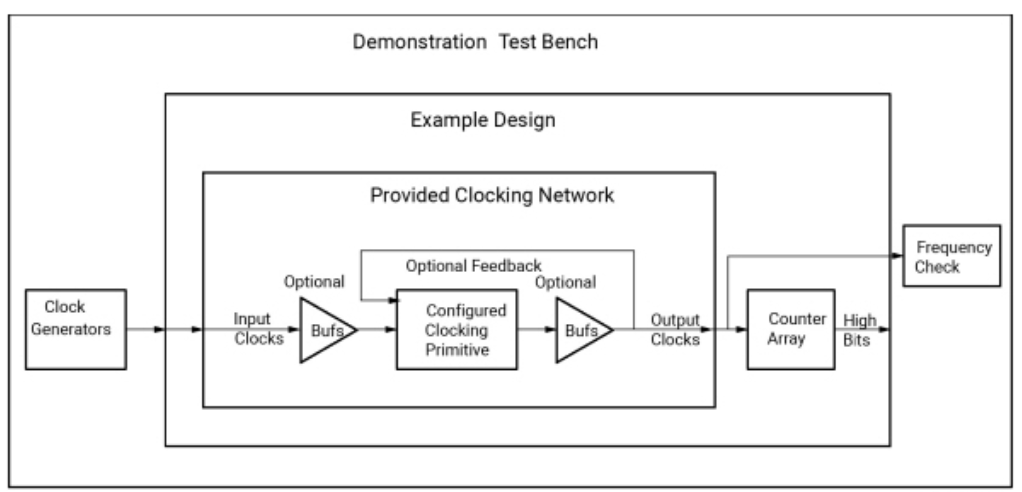
\includegraphics[width=0.85\textwidth]{gfx/diagrams/Clocking_Wizard_BlockDiagram.png}
	\caption{Clocking Wizard Block Diagram \cite{xilinx_clocking_wizard}}
	\label{fig:technical_background:Clock_Nuances_ClockingWizard}
\end{figure}

While the Clocking Wizard simplifies clock creation, the presence of multiple independent clocks introduces a new challenge: clock domain crossing (CDC). \acs{CDC} problems happen when signals that are not synchronized move between different clock domains. This can cause metastability, leading the design to behave unpredictably. In some cases, metastability can cause excessive current and even damage the chip. Because the delay for signals crossing between clock domains cannot be guaranteed, this unpredictability is a concern \cite{IEEE_CDC}. To prevent these issues, it is important to thoroughly test designs with multiple clock domains and ensure \acs{CDC}-related problems do not affect system operation.

One way to mitigate the \acs{CDC} when two different clock frequencies are involved in an \acs{FPGA} Design is to use Xilinx \acs{CDC} \acs{IP} core. An example implementation of this approach is illustrated in the accompanying figure \ref{fig:clock_example}. The Clocking Wizard module (clk\_wiz\_1) generates a 192 MHz clock signal derived from the 100 MHz system frequency. This 192 MHz output drives the debugger \acs{IP} for on-chip signal monitoring and debugging.

The \acs{PWM} generator module generates \acs{PWM} signals at 100 MHz, the system clock frequency. Because the debugger module operates at 192 MHz, direct capture of the \acs{PWM} signals is not possible due to the differing clock domains. To synchronize these signals, the Xilinx \acs{CDC} \acs{IP} Core (xpm\_cdc\_gen\_3) is inserted between the \acs{PWM} generator module and the debugger.

The \acs{CDC} \acs{IP} core receives the source clock (100 MHz), the destination clock (192 MHz), and the source signal (\acs{PWM} output). It generates a synchronized version of the input signal, aligned with the destination clock domain. This synchronized signal is routed to the debugger, enabling reliable signal capture without metastability.

This configuration ensures that signals transferred from the \acs{PWM} generator module at 100 MHz are safely synchronized and observable in the 192 MHz domain used by the debugger module. As a result, the design maintains deterministic and stable behavior across multiple clock domains.

\begin{figure}[htbp]
	\centering
	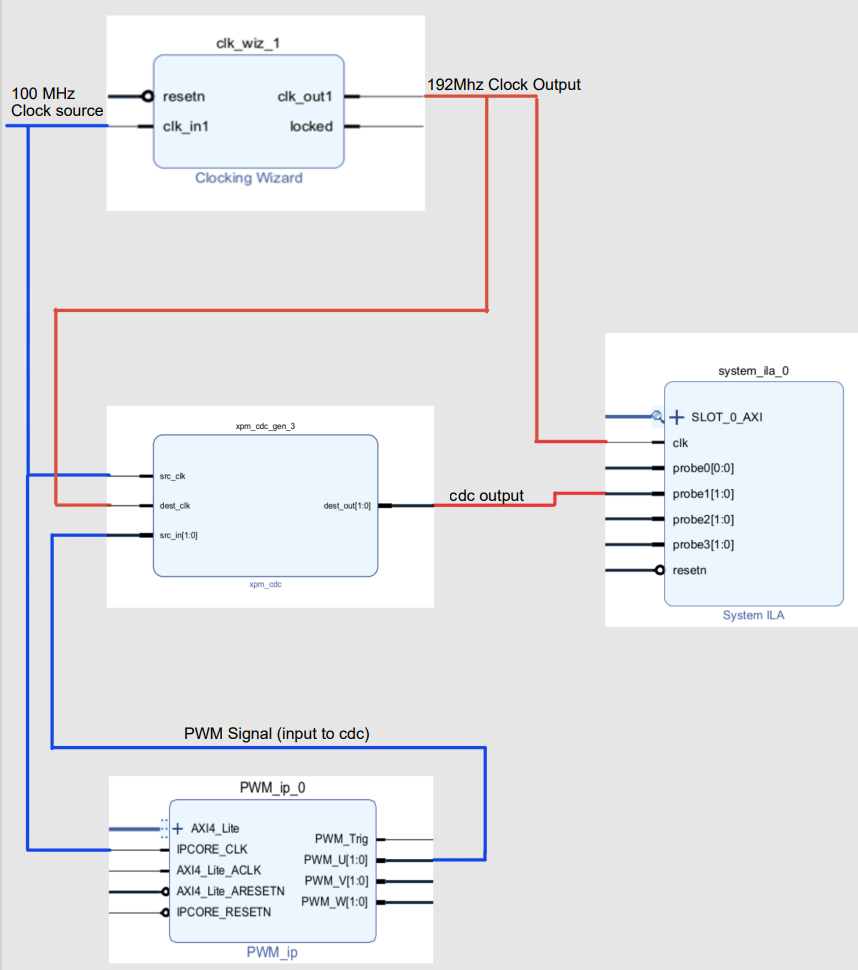
\includegraphics[width=\textwidth]{gfx/diagrams/clock_Nuances.png}
	\caption{An example illustrating the use of Clocking Wizard and Xilinx \acs{CDC} \acs{IP} Core}
	\label{fig:clock_example}
\end{figure}

%\begin{center}
%	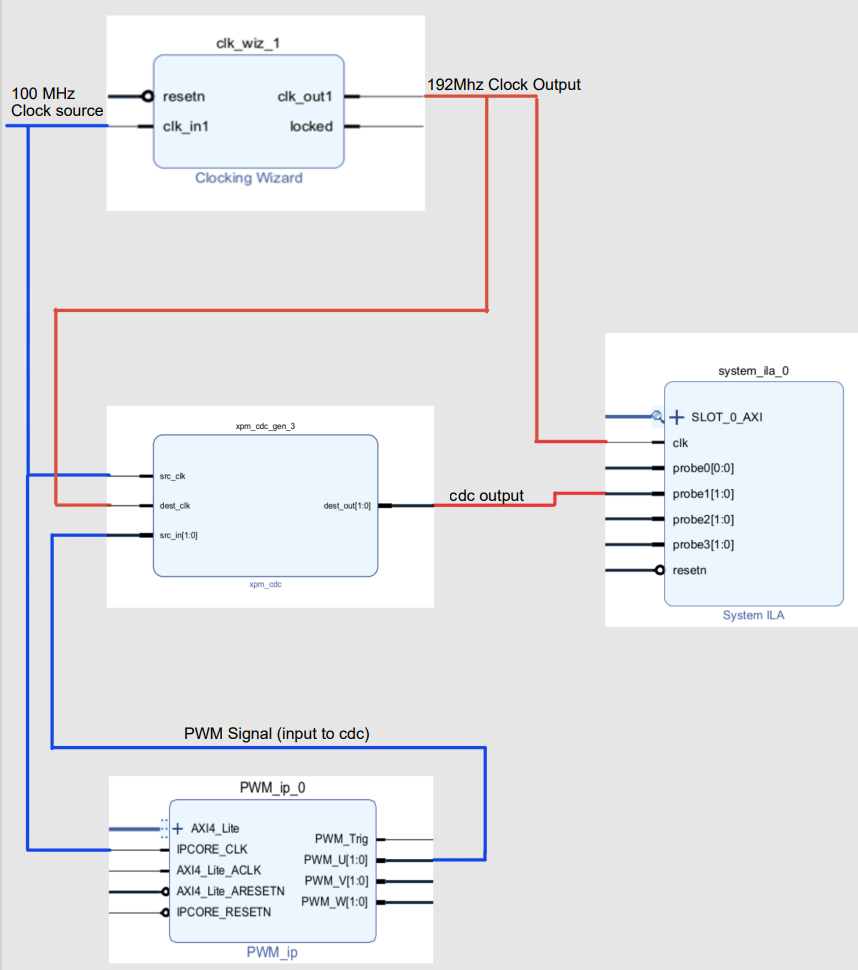
\includegraphics[width=\textwidth]{gfx/diagrams/clock_Nuances.png}
%	\captionof{figure}{An example illustrating the use of Clocking Wizard and Xilinx CDC IP Core}
%	\label{fig:clock_example}
%\end{center}

Effective clock management is essential in designs with multiple clock domains to ensure correct operation and address specific verification challenges. Signal transfers between asynchronous domains, even when using \acs{CDC} \acs{IP} cores for synchronization, can result in subtle timing and functional issues that are difficult to detect. As \acs{FPGA} designs become more complex, with higher speeds and diverse processing elements, comprehensive verification is required to maintain reliable, predictable performance. The following section examines several \acs{FPGA} verification methods, including simulation, in-system testing, and hardware-in-the-loop approaches, which facilitate the identification and resolution of timing and functional issues in modern \acs{FPGA} designs.

\section{Types of \acs{FPGA} Verification}
\label{sec:TechBackground:Types_of_FPGA_Verification} 

\vspace{-0.50\baselineskip}
Verifying \acs{FPGA} designs involves specific tasks and tools tailored to the technology. Unlike ASIC designs, \acs{FPGA} implementations typically lack extensive verification resources and dedicated planning. Often, verification is treated as secondary because \acs{FPGA}s can be reprogrammed. Neglecting comprehensive verification planning may result in substantial development delays and disruptions, which are comparable to the setbacks caused by unexpected technology re-spins. Assuming verification is low-risk because errors can be corrected by reprogramming overlooks the effort required to identify and resolve issues, especially in complex designs featuring multiple clock domains. Delays in hardware verification can also affect other development areas, such as software and system integration, due to their interdependence \cite{Bouldin2006_FPGA}.

A structured hierarchy of verification methodologies helps reduce \acs{FPGA}-related risks. Initial verification focuses on identifying major functional issues at a high level. As the process advances toward a fully operational, high-speed design, errors become more subtle and are often related to timing or specific data conditions. Some issues are so rare they may only appear after extended operation. In these cases, the test environment must capture enough information for thorough analysis and resolution \cite{Bouldin2006_FPGA}.


\subsection{Simulation Verification}
\label{sec:TechBackground:Simulation_Verification} 

In \acs{FPGA} functional verification, simulation plays a vital role in the design process. It enables engineers to model and evaluate digital circuits prior to hardware implementation, helping to detect design flaws and confirm correct operation. Through simulation, mathematical representations of \acs{FPGA} systems are created, various test scenarios are applied, and the 
resulting outputs are analyzed. 

This approach provides valuable insights into system behavior, assists in performance evaluation, and supports validation of design choices. A solid understanding of simulation principles allows designers to optimize \acs{FPGA} architectures, minimize development risks, and enhance the overall reliability and robustness of digital systems \cite{Cui2024_FPGA}. \newline
\vspace{0.35\baselineskip}	
\begin{figure}[H]
	\centering
	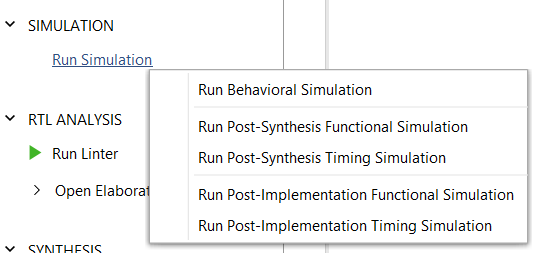
\includegraphics[width=0.65\textwidth]{gfx/diagrams/Types_of_simulation.png}
	\caption{Types of \acs{FPGA} Simulation Verification}
	\label{fig:technical_background:SimulationVerification}
\end{figure}
The figure above illustrates the various existing simulation verification methods.
\begin{itemize}
	\item \textbf{Behavioral / RTL Simulation: }
	RTL-level simulation enables simulation and verification of a design before translation by synthesis or implementation tools. Designs can be verified at the module, entity, block, device, or system level.
	
	RTL simulation is typically conducted to verify code syntax and confirm correct functionality. At this stage, the design is described in RTL, and timing information is not required \cite{AMD_VivadoSimUG900}.
	
	There are two main approaches to behavioral or RTL simulation. The first uses event-driven execution, where the simulator processes generated code based on events. The second is a compiled simulation, which executes the code directly at specific time points. Compiled simulation supports only zero-delay scenarios and assumes the circuit is synchronous. In both methods, statements at lower levels are executed sequentially, while at the module level, execution is event-driven. For example, statements within a VHDL process block are executed sequentially \cite{IEEE_ICVD1993}.
	
	\item \textbf{Post Synthesis Simulation: }
	A synthesized netlist is generally simulated to verify that the design fulfills functional requirements and exhibits the intended behavior. Timing simulation using estimated timing values may also be conducted at this stage, although this practice is less common.
	
	The functional simulation netlist is organized hierarchically and folded, with expansion down to the level of primitive modules and entities\cite{AMD_VivadoSimUG900}.
	
	\item \textbf{Post Implementation Simulation: }
	After implementation, either functional or timing simulation may be performed. Timing simulation most accurately replicates the process of downloading a design to a device. This method verifies that the implemented design meets both functional and timing requirements and demonstrates the expected behavior within the device\cite{AMD_VivadoSimUG900}.
\end{itemize}

\subsection{In-System Verification}
\label{sec:TechBackground:In_System_Verification} 

Embedded logic analyzers provide the capabilities of traditional external logic analyzers but are implemented within the \acs{FPGA} fabric using dedicated \acs{IP} cores that connect to specific internal signals. These analyzers capture signal activity according to user-defined trigger conditions and store the resulting data in on-chip memory for subsequent analysis. Although some runtime configuration is possible, most trigger conditions and signal selections are established during the design phase. Debug cores require \acs{FPGA} resources, particularly block RAMs for trace storage, and modifications to the instrumentation typically necessitate re-synthesizing the design. Nevertheless, embedded logic analyzers offer near real-time signal visibility and can function at or near the target system frequency.

\begin{figure}[htbp]
	\centering
	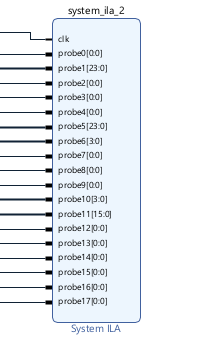
\includegraphics[width=0.30\textwidth]{gfx/diagrams/System_ILA.png}
	\caption{System \acs{ILA} \acs{IP} Core}
	\label{fig:technical_background:System_ILA}
\end{figure}

Earlier toolchains featured Xilinx ChipScope Pro and Intel (formerly Altera) SignalTap II as primary examples of embedded logic analyzer solutions. In current workflows, ChipScope Pro has been replaced by the Vivado Integrated Logic Analyzer and System \acs{ILA} \acs{IP} (Figure \ref{fig:technical_background:System_ILA}) from AMD (Xilinx), while SignalTap II continues as Intel’s integrated solution for Quartus-based designs. Additional tools, including the Synopsys Identify RTL Debugger, offer advanced source-level instrumentation and debugging capabilities for \acs{FPGA} development.

%A second major approach involves JTAG-based inspection and capture. These tools acquire device state snapshots via boundary-scan access, eliminating the need for embedded instrumentation and preserving FPGA resources. They provide comprehensive visibility into register and configuration data, but are constrained by the limited data throughput of the JTAG interface. As device complexity increases, the time required to extract a complete device state also rises. Historically, tools such as Xilinx JBits and BoardScope offered research-grade JTAG inspection capabilities, though both are now discontinued. Modern alternatives include AMD’s Vivado Hardware Manager, which uses JTAG to configure, control, and retrieve data from on-chip debug cores, as well as vendor-agnostic solutions like Exostiv Labs’ EXOSTIV, which increase capture bandwidth by streaming internal FPGA activity through dedicated high-speed transceivers.

\subsection{Software-Driven Verification}
\label{sec:TechBackground:Software_Driven_Verification} 

Software-driven verification is an advanced methodology for \acs{FPGA} validation that utilizes embedded processors within the \acs{FPGA}, such as ARM cores in Xilinx Zynq, MicroBlaze soft processors, or Intel Nios II, to validate hardware modules using executable test software. In this methodology, the processing system executes test routines or firmware that interact with the programmable logic via standard on-chip communication interfaces such as AXI4-Lite (Figure \ref{fig:technical_background:Software-Driven Verification}) or AXI4-Stream. This approach enables real-time verification of design functionality under realistic operating conditions and serves as a bridge between pre-silicon verification and post-silicon validation \cite{IEEE10488040}. The \acs{PS} configures, stimulates, and monitors \acs{PL} blocks by reading and writing \acs{AXI}-mapped control and status registers, while embedded test software automates both functional and performance verification sequences.

%\vspace{0.35\baselineskip}
\begin{figure}[H]
	\centering
	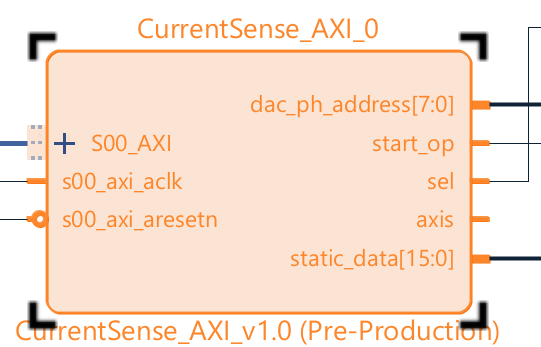
\includegraphics[width=0.46\textwidth]{gfx/diagrams/AXI_Interface.png}
	\caption{An example for AXI4 \acs{IP} Core}
	\label{fig:technical_background:Software-Driven Verification}
\end{figure}

Software-driven verification is increasingly adopted in modern \acs{SoC}-FPGAs due to its flexibility and scalability. This methodology accelerates verification and enhances design observability and performance monitoring \acs{IP} cores. As shown in recent \acs{IEEE} research, frameworks such as HIVE \cite{IEEE10488040} demonstrate that running test software on embedded processors significantly improve coverage for hardware and software interaction, \acs{AXI} protocol compliance, and timing validation across the \acs{PS}–\acs{PL} boundary by running test software on embedded processors

\subsection{Hardware-in-loop Verification}
\label{sec:TechBackground:HIL_Verification} 

Traditional software-based simulation is limited in its ability to replicate operational conditions. Hardware-in-the-loop (HIL) simulation mitigates this limitation by integrating real hardware components into the simulation environment. In real-time \acs{HIL} simulation, physical hardware replaces emulated hardware or control logic within the simulation model and interacts directly with computational models. This method increases simulation fidelity, provides access to hardware-specific features not present in software-only models, and decreases the likelihood of undetected errors during final field testing \cite{HIL}.

A special subset of \acs{HIL}, known as \textbf{\acs{FPGA}-in-the-Loop (FIL)} verification, focuses on integrating \acs{FPGA}-based designs as the device under test (DUT) within the simulation environment. The \acs{DUT} is implemented on a physical \acs{FPGA}, while a separate hardware platform, such as another \acs{FPGA} or a real-time controller, supplies input signals and captures output responses for analysis. This setup enables real-time verification of \acs{FPGA} logic for both functional correctness and timing accuracy. Unlike full \acs{HIL}, \acs{FIL} does not simulate physical system dynamics but instead offers a high-fidelity environment for testing \acs{FPGA} modules with precise synchronization and low latency, which is especially valuable for high-speed digital systems.

A review of \acs{FPGA} verification methods demonstrates that real-time observation of internal signals is critical for debugging and validating complex designs. Although simulation and software-based verification are valuable, specific timing behaviors, particularly in systems with multiple clock domains, are observable only on physical hardware. The \acs{ILA} \acs{IP} Core fulfills this requirement by offering on-chip tools for real-time signal monitoring. These tools enable designers to detect and resolve subtle functional and timing issues. The following section describes the \acs{ILA}’s types, features and practical applications in \acs{FPGA} design and verification.

\section{System Integrated Logic Analyzer}
\label{sec:TechBackground:SystemILA} 

\vspace{-1.0\baselineskip}
The Integrated Logic Analyzer (ILA) is a built-in debug \acs{IP} core provided by Xilinx that allows in-system probing of internal \acs{FPGA} signals. Rather than routing signals out to external pins, the \acs{ILA} captures internal signal waveforms in on-chip memory (e.g. BRAM / UltraRAM) and then makes them available for visualization.

The System \acs{ILA} \acs{IP} is a recent solution intended for block designs and systems that use an \acs{IP} integrator or \acs{SoC} architecture. This tool enables the probing of protocols such as AXI4 and \acs{AXI} Stream, and provides enhanced integration with Vivado debug tools.

In \acs{FPGA} design, signals and interfaces are connected to the System \acs{ILA} using probe and slot inputs, as illustrated in figure. These signals and interfaces are sampled at the design's operating frequency and stored in on-chip Block RAM (BRAM) \cite{Xilinx_SystemILA}. 

Communication with the System \acs{ILA} core is established through an automatically generated debug core hub that connects to the \acs{FPGA} \acs{JTAG} port. After programming the design into the \acs{FPGA}, the Vivado Hardware Manager software enables configuration of trigger events for System \acs{ILA} measurements. When the trigger condition is met, the sample buffer collects data and transmits it to the Hardware Manager for visualization and analysis in the waveform window \cite{Xilinx_SystemILA}.

\begin{figure}[htbp]
	\centering
	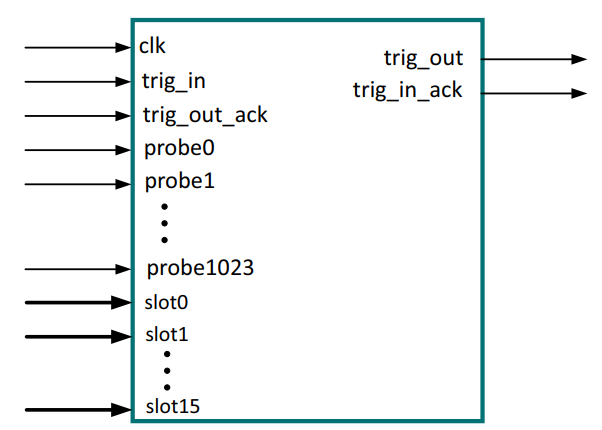
\includegraphics[width=0.70\textwidth]{gfx/diagrams/System_ILA_Symbol.png}
	\caption{System \acs{ILA} Symbol \cite{Xilinx_SystemILA}}
	\label{fig:technical_background:System_ILA_Symbol}
\end{figure}

%\vspace{-3.0\baselineskip}
Standard \acs{FPGA} logic manages probe sampling and trigger operations, while on-chip BRAM temporarily stores captured data until the software retrieves it. The process, encompassing triggering, data capture, and communication with the System \acs{ILA} core, operates automatically without requiring user intervention \cite{Xilinx_SystemILA}.

The System \acs{ILA} can monitor interface-level signals, providing transaction-level insights, such as tracking outstanding transactions on AXI4 interfaces. This feature establishes the System \acs{ILA} as a valuable tool for analyzing \acs{AXI}-based communication in \acs{FPGA} and \acs{SoC} designs. The System \acs{ILA} captures and displays AXI4 transactions in real time, enabling verification of protocol compliance, observation of data flow between master and slave components, and identification of potential bottlenecks or design issues. Effective use of the System \acs{ILA} for monitoring and debugging requires a thorough understanding of \acs{AMBA} \acs{AXI} interfaces.

The figure \ref{fig:technical_background:System_ILA_AXI} presents a practical example of the System \acs{ILA} capturing AXI4 write transactions. The waveform displays key \acs{AXI} signals, including \textbf{AWVALID}, \textbf{AWREADY}, and \textbf{AWADDR}, demonstrating the \acs{ILA}'s capability to provide real-time visibility into the transaction process and to support verification of correct protocol operation.


\begin{figure}[htbp]
	\centering
	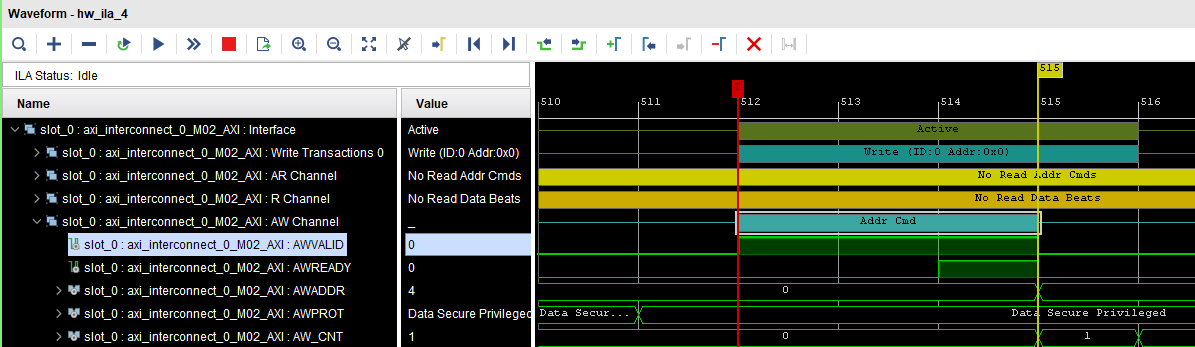
\includegraphics[width=1.00\textwidth, height=0.3\textheight]{gfx/diagrams/AXI_ILA.png}
	\caption{System \acs{ILA} capture of AXI4 write transaction signals.}
	\label{fig:technical_background:System_ILA_AXI}
\end{figure}


\section{\acs{AMBA} \acs{AXI} Interfaces}
\label{sec:TechBackground:AXI_INterfaces} 

The ARM Advanced Microcontroller Bus Architecture (AMBA) is an open standard specification for on-chip communication and interconnection that manages functional blocks within a \acs{SoC} design. The \acs{AMBA} protocols define the mechanisms that enable communication between these functional blocks \cite{Introduction_to_AMBA}.

The Advanced eXtensible Interface (AXI) constitutes the third generation of the \acs{AMBA} standard, introduced in the \acs{AMBA} 3 specification. \acs{AXI} is designed for systems that demand high performance and rapid clock speeds, incorporating features that enable efficient, high-speed interconnects in sub-micrometer technologies. In 2010, ARM introduced the \acs{AMBA} 4 specifications, beginning with AXI4, and subsequently released the \acs{AXI} Coherency Extensions (ACE) in 2011 to improve system coherency. The AXI4-Stream protocol enables unidirectional data transmission from the manager to the subordinate. Its simplified signal routing makes it especially suitable for implementation in \acs{FPGA}-based systems \cite{Introduction_to_AMBA}.

The \acs{AXI} protocol specifies the processes for reading, writing, caching data, and translating addresses. These operations utilize several distinct communication channels \cite{AXI_INTERFACES}:

\begin{itemize}
	\item Write request signals are denoted by the prefix \textbf{AW}.
	\item Write data signals are denoted by the prefix \textbf{W}.
	\item Write response signals are denoted by the prefix \textbf{B}.
	\item Read request signals are denoted by the prefix \textbf{AR}.
	\item Read data signals are denoted by the prefix \textbf{R}.
\end{itemize}

\begin{figure}[htbp]
	\centering
	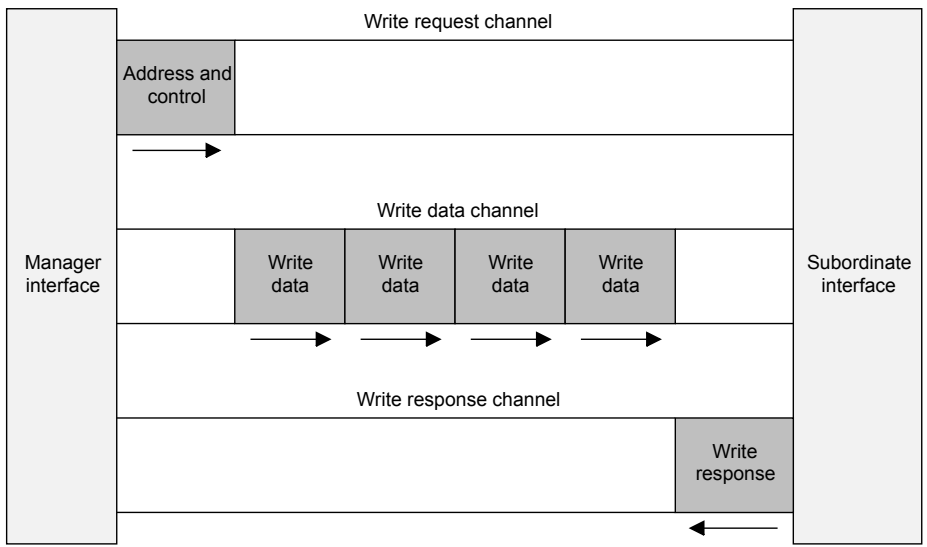
\includegraphics[width=1.00\textwidth]{gfx/diagrams/AXI_WRITE.png}
	\caption{The figure illustrates the operation of a write transaction, which utilizes the write request, write data, and write response channels \cite{AXI_INTERFACES}.}
	\label{fig:technical_background:AMBA_AXI_WRITE}
\end{figure}

A request channel transmits control information specifying the type of data to be transferred. Data is exchanged between the Manager and Subordinate through the following channels \cite{AXI_INTERFACES}:

\begin{itemize}
	\item \textbf{Write data channel:} The Manager transmits data to the Subordinate via this channel. Upon completion, the Subordinate notifies the Manager through the write response channel.
	\item \textbf{Read data channel:} The Subordinate transmits data to the Manager through this channel.
\end{itemize}

\begin{figure}[htbp]
	\centering
	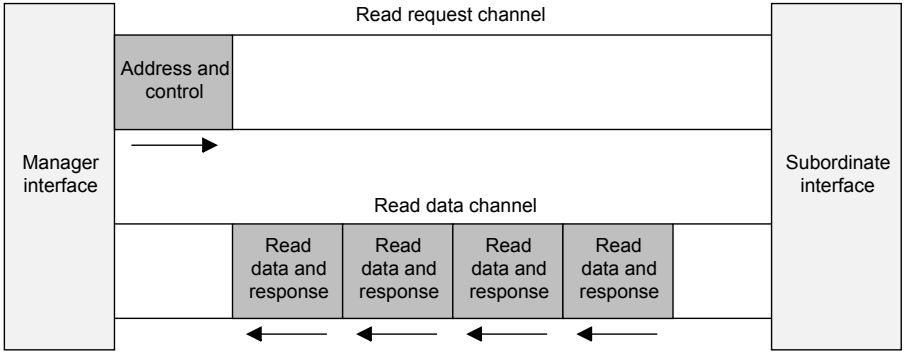
\includegraphics[width=1.00\textwidth]{gfx/diagrams/AXI_READ.png}
	\caption{The figure depicts a read transaction, demonstrating the use of the read request and read data channels \cite{AXI_INTERFACES}.}
	\label{fig:technical_background:AMBA_AXI_READ}
\end{figure}

\textbf{Write and Read Request Channels}

The \acs{AXI} protocol specifies separate channels for write and read requests. Each channel transmits the address and control information required to initiate a transaction.

\textbf{Write Data Channel}

The write data channel transfers data from the Manager to the Subordinate, supporting data widths up to 1024 bits. A byte-lane strobe signal indicates valid bytes for every eight bits. Data on this channel is always buffered, allowing the Manager to initiate multiple write transactions consecutively without waiting for confirmation from the Subordinate.

\textbf{Write Response Channel}

The Subordinate utilizes the write response channel to indicate completion of a write transaction. Each transaction requires a completion signal on this channel. As illustrated in Figure \ref{fig:technical_background:AMBA_AXI_WRITE}, the response is provided only after the entire transaction is complete, rather than after each data segment.

\textbf{Read Data Channel}

The read data channel transmits both read data and response information from the Subordinate to the Manager. Similar to the write data channel, it supports data widths up to 1024 bits.

\textbf{\acs{AXI} Interface Variants}

The \acs{AMBA} \acs{AXI} comprises three primary types. Each variant provides a distinct balance between complexity and performance to address diverse design requirements \cite{Xilinx_AXI}.

\begin{itemize}
	\item AXI4 (Full) is a high-speed, memory-mapped interface that supports burst transfers of up to 256 beats, enables concurrent transactions, and manages out-of-order responses. These features make it suitable for memory-intensive applications.
	\item AXI4-Lite is a simplified version of AXI4 that supports basic single-read or single-write operations. It is typically used for control and status registers, where resource efficiency is prioritized over speed.
	\item AXI4-Stream is a unidirectional, high-speed streaming interface that omits the address phase and utilizes only data and handshake signals. It is commonly implemented in real-time data pipelines such as video processing, digital signal processing, and communication systems.
\end{itemize}

Collectively, these three interface types establish a flexible interconnect system. AXI4 connects to main memory, AXI4-Lite handles configuration and control, and AXI4-Stream facilitates continuous data flow. This architecture ensures consistent integration across intellectual property cores in Vivado-based system-on-chip designs\cite{AXI_INTERFACES}\cite{Xilinx_AXI}.

The technical elements presented in this chapter constitute the primary components of the proposed verification platform. With the theoretical foundation established, the subsequent chapter will detail the concepts and models used to design the platform’s architecture and demonstrate how these technologies contribute to a robust, automated solution for \acs{PL} module verification.

